% Chapter 1

\chapter{Introduction} % Main chapter title
\label{sens_introduction} % For referencing the chapter elsewhere, use \ref{sens_introduction} 


3D reconstruction aims to reproduce the 3D profile of real objects as accurate as possible, which require accurate world X/Y/Z (noted as \(X_{w}\) /\(Y_{w}\) /\(Z_{w}\)  henceforth) coordinate values in three dimensional space for every single point of a profile. Ever since the Kinect brought low-cost depth cameras into consumer market, with PrimeSense 3D sensing technology as the core depth determination principle for its first generation, great interest has been invigorated into RGB-D sensors. Camera calibration is a necessary part in 3D reconstruction in order to extract metric information from 3D images, i.e., to determine a translation from \(Z_{w}\)  to \(X_{w}\) /\(Y_{w}\)  for every pixel based on its row and column. In the mean time, optical and perspective distortion become a problem that stops from getting a good view. On most wide angle prime lenses and many zoom lenses with relatively short focal lengths,  especially cheap low quality lenses, barrel distortion would typically be present.
\\
\\In this research, a more accurate novel method with precise calibration system is brought in for real-time rectification and 3D reconstruction of universal RGB-D cameras. 
%%%%%%%%%%%%%%%%%%%%%%%%%%%%%%%%%%%%%%%%%%%%%%%%%%%%%%%%%%
%%%%%%%%%%                                                     %%%%%%%%%%%%%%%%%%%%%%%%%%%%%%%%
%%%%%%%%%% 1.1   3D Reconstruction                   %%%%%%%%%%%%%%%%%%%%%%%%
%%%%%%%%%%                                                     %%%%%%%%%%%%%%%%%%%%%%%%
%%%%%%%%%%%%%%%%%%%%%%%%%%%%%%%%%%%%%%%%%%%%%%%%%%%%%%%%%%%%
\section{3D Reconstruction}
Three dimensional (3D) profile measurement technologies have been developed by various means, as summarized by Curless and Seitz [1], % B. Curless and S. Seitz, \3d photography," ACM Siggraph '00 Course Notes, Course No. 19 (2000).
among which the non-contact optical methods are widely applied into reality as consumer RGB-D camera. Traditionally, with Pinhole camera model, as the basics of camera calibration, to supply the translation from \(Z_{w}\)  to \(X_{w}\) /\(Y_{w}\) , the core procedure of 3D Reconstruction falls on the determination of per-pixel depth to serve as \(Z_{w}\) .
%
 \\\\Figure 1.1\\\\
Within the non-contact optical category, as well as 3D reconstruction using multiple images, there are two levels of distinctions[2],
% 3D Reconstruction from Multiple Images.pdf
 as shown in the 3D profile acquisition taxonomy diagram is given in Figure 1.1.% the branch tree diagram
 %
 \\\\The first distinction: active methods and passive methods. Their classifications are decided by the control of light sources. Active methods need special light sources control as part of the strategy to get 3D information, while on the other hand, passive techniques could work with whichever reasonable available ambient light. With a special known illumination offering more information to simplify some of the steps for 3D information acquiring process, active methods tend to be computationally less demanding. Both of the famous consumer PrimeSense and Kinect V2 3D cameras, which are calibrated by the new proposed approach, are using active methods.
\\\\The second distinction: single-vantage points methods and multi-vantage points methods. The second distinction is determined by the number of vantage points. With a single vantage system, reconstruction is done based on single view point. In the case that there are multiple viewing or illumination components, all of them would be positioned very close to each other so that they could ideally coincide. For multi-vantage points methods, several viewpoints, with possible controlled illumination source positions, are involved. As contrast with the single-vantage points methods, the multi-vantage systems need the different components to be positioned far enough from each other. 
\\ \\
Among the above non-contact optical methods, structured-light and time-of-flight methods are of the most practical importance.
As will be discussed shortly, the PrimeSense technology and SeikowaveLCG camera use Stuctured light methods, and the Kniect V2 camera uses Time-of Flight. 
\\
\\\textbf{Structured Light}\\\\
Structured light (SL) based techniques are famous for its fast speed. It is composed of one camera and one light pattern projector[3]. %Real-time 3-D Reconstruction by Means of Structured Light Illumination
The projector projects a series of special known patterns onto a target, and the camera captures the corresponding images, which contain special information corresponded to the patterns from the projector. A decoding algorithm would be used to extract world coordinate information of the target object from the captured images, by analyzing the relationship among the camera, the projector and the target object using triangulation.\\
\\
Being after accuracy, the most important issue for structured light method comes to the question of, how to design the projected patterns. In other words, how to design the coding algorithm and its corresponding decoding strategy will decide the final quality of the reconstructed 3D profile. Various classified SL pattern strategies have been proposed, and are still being studied.
\\
\\\textbf{PrimeSense SL speckle pattern}\\\\
The PrimeSense 3D camera uses an infrared projector to project an infrared speckle pattern onto a target 
% RGBD-intro.pdf/   Consumer RGBD Cameras and their Applications
, as shown in figure 1.2,%Figure1 in the pdf named above
\\\\Figure 1.2\\\\
and an infrared camera to capture images of the target. By comparing part by part to reference patterns, that were captured previously at known depths and stored in the device, the per-pixel depth could be looked up based on the reference pattern that the projected pattern matches best. 
\\\\
After the per-pixel depth data determined from the infrared sensor, the next step would be to correlate to a calibrated RGB data, which will generate a popular unified representation of target's profile: point cloud, a collection of points with XYZ 3D coordinates and RGB color data. What's more, the surface normals of the target's profile are also stored in every single point of the point cloud data. 
\\
\\\textbf{Seikowave SL Phase Measuring Profilometry pattern}\\\\%triangulation
SeikowaveLCG 3D camera consists of a Charge-Coupled Device (CCD) camera and a Digital Micro-mirror Device (DMD) projector. 2D image pattern strategies are always preferred for a fast scan if a is involved. 
[4]%J. Salvi, J. Pages, and J. Batlle, \Pattern codication strategies in structured light systems," Pattern Recognition 37, 827{849 (2004).
 [5] %  ''Novel method for structured light system calibration'' SongZhang
And the multi-shot pattern Phase Measuring Profilometry (PMP) strategy was used for its properties of robust and accuracy.
With PMP information encoded in the structured light pattern projected onto the target, the CCD camera could capture a series of images that contains PMP informatio. Triangulation analyzing could be used to extract the 3D world coordinates for each points of the target profile, by a determination of the relationships among CCD camera, DMD projector, and the target object. A system configuration of PMP application is given in figure 1.3.
 \\\\Figure 1.3\\%Fig. 8 Structured light system configuration/  in paper [5]
 \\
 PMP  method uses either vertical or horizontal sinusoid patterns, which could be described as:\\
 (Projector) In(x, y) = A + B*Cos(2pi*f*y - 2pi*n/N)	   (1.1)% equation 1.1 in Kai's paper
 \\where (xp, yp) denotes the coordinates of every single pixel in the projector, In denotes the intensity of the corresponding pixels, Ap and Bp are constants, f is the frequency of sine wave. The subscript n represents the index of phase shift, while capital N is the total number of phase shift. Figure 1.4 below shows a group of sine wave patterns, where the number of total phase shift N = 4 and frequency f = 1.\\
 \\Figure 1.4\\%Figure 1 : PMP base frequency patterns/ in paper [6]
\\
From viewpoint of the camera, the sinusoid patterns is distorted by the target surface topology, so that the captured images could be expressed as 
(Camera)    In(x, y) = A + B*Cos(Phi(xc,yc) - 2pi*n/N)    (1.2)%equation 1.2 in Kai's paper
\\where (xc, yc) denotes the coordinates of every single pixel in the camera, and the term Phi(xc, yc) represents the corresponding phase value, which could be computed as follows [6]\\
 % Very High Resolution 3-D surface Scanning Using Multi-Frequency Phase Measuring Profilometry
Phi(xc, yc) =arctan[]		(1.3) % equation 3 in paper [6]
\\After the camera term phi(xc, yc) for every single pixel is computed, the corresponding projector coordinate yp could be derived through equation\\
yp = phi/2pi*f		(1.4)%equation 4 in paper [6]
\\With the knowledge of yp, the perspective information between camera and projector is the last step to go for applying triangulation analysis to extract world coordinates. Based on pinhole camera model, the perspective matrices for camera and projector are [7]\\
% J. Li, L. G. Hassebrook, and C. Guan, \Optimized two-frequency phasemeasuring-prolometry light-sensor temporal-noise sensitivity," Journal of the Optical Society of America A 20, 106{115 (2003).
Mc = () 		(1.5) %equation 1.9 in Kai's paper
\\and \\
Mp = ()		(1.6)%equation 1.10 in Kai's paper
\\The transforms from 3D world coordinates to 2D camera coordinates are given by\\
xc = \textendash		(1.7)\\%equation 1.11 in Kai's paper
yc = \textendash\ 	(1.8)\\%equation 1.12 in Kai's paper
\\Likewise, the map from 3D world coordinates to 2D projector coordinates are given by\\
xp = \textendash		(1.9)\\%equation 1.13 in Kai's paper
yp = \textendash\ 	(1.10)\\%equation 1.14 in Kai's paper
\\
Since three out of four equations (1.7 \~{} 1.10) are enough to solve \(X_{w}\) , \(Y_{w}\) , and \(Z_{w}\) , and yp is already calculated, the 3D world coordinates \(X_{w}\) /\(Y_{w}\) /\(Z_{w}\)  could be derived from Eqs 1.7, 1.8, 1.10\\
() = () ()			(1.15)%equation 1.15 
\\
\\
\\\textbf {Time of Flight}\\
 Based on known speed of light, Time-of-Flight (ToF) camera resolves distance by measuring the time cost of a special light signal traveling between the camera and target for every single point. Kinect V2 is one of the practical consumer 3D camera that applied the technology of ToF. Using the active modulated infrared source light together with a low-cost CMOS pixel array, Kinect V2 realize its an attractive solution that owns compact construction, high accuracy and up to 30 fps frame-rate. \\
  \\\\Figure 1.5\\\\%Fig. 1: 3D time-of-flight camera operation /  in paper [8]
 The variable that ToF camera measures is the phase shift between the illumination and reflection, which will be translated to distance [8]. % Texas Instruments Time-of-Flight Camera -An Introduction    Larray Li
To detect the phase shifts, light source is pulsed or modulated by a continuous wave, typically a sinusoid or square wave.
As figure 1.5 shows, the ToF camera illumination is typically from a LED or a solid-state laser operating in the near-infrared range invisible to human eyes. A camera working in the same spectrum captures the reflected light and converts photonic energy to electrical signal, which contains distance (depth) information.
\\\\
The distance measured for every single pixel is saved into a 2D addressable array, which results in a depth map. Kinect V2 has a depth map of 512 * 424 unsigned short data collections, which could be finally rendered, together with corresponded RGB stream,  into a tree dimensional space point cloud.
%%%%%%%%%%%%%%%%%%%%%%%%%%%%%%%%%%%%%%%%%%%%%%%%%%%%%%%%%%
%%%%%%%%%%                                                     %%%%%%%%%%%%%%%%%%%%%%%%%%%%%%%%
%%%%%%%%%%  1.2   Traditional RGB-D camera calibration                   %%%%%%%%%%%%%%%%%%%%%%%%
%%%%%%%%%%                                                     %%%%%%%%%%%%%%%%%%%%%%%%
%%%%%%%%%%%%%%%%%%%%%%%%%%%%%%%%%%%%%%%%%%%%%%%%%%%%%%%%%%%%
\section{Traditional RGB-D camera calibration} % (specially with cheap low quality lenses)
\label{sens_TraditionalCalibration} % For referencing the chapter elsewhere, use \ref{sens_TraditionalCalibration} 
Traditionally, camera calibration consists of two parts: ideal pinhole camera model calibration, and lens distortion correction. The pinhole camera model works as an simple algorithm in 3D computer vision to describe a mapping from the 3D world coordinates to camera image row and column, thereby giving a translation method from \(Z_{w}\) to \(X_{w}\)  and \(Y_{w}\)  for every single pixel. It works decently only for ideal pinhole cameras that have no lens, whereas real cameras need extra modifications and supplementations. In order to accurately solve the non-linear distortions problem for a real camera, the second part radial and tangential lens distortion must be considered.\\\par

\subsection{Pinhole Camera Model}
%%
Figure \ref{PinholeCameraModel} shows the basic diagram of a pinhole camera model with a reflected image plane for friendly intuition
[9].% Short on camera geometry and camera calibration/ Maria Magnusson
From this model, the mapping between 3D space world coordinate and the image plane row and column could be separated into two parts of transformations. The first part is the transformation between world coordinates system \(X\)/\(Y\)/\(Z\) and camera coordinate system \(U\)/\(V\)/\(W\) , which forms a 4-by-4 perspective transformation matrix (\textbf{extrinsic calibration}) that works for 3D rotation and translation. And the second part is the mapping between 3D camera coordinates system \(U\)/\(V\)/\(W\) and 2D image plane coordinates  \(u\)/\(v\), which forms a 3-by-3 perspective transformation matrix (\textbf{intrinsic calibration}) that works for not only the rescaling between camera coordinates and virtual ideal image coordinates, but also for translating and skewing between the virtual ideal image plane and real image plane.  \\\\\par

\begin{figure}[h]
\centering
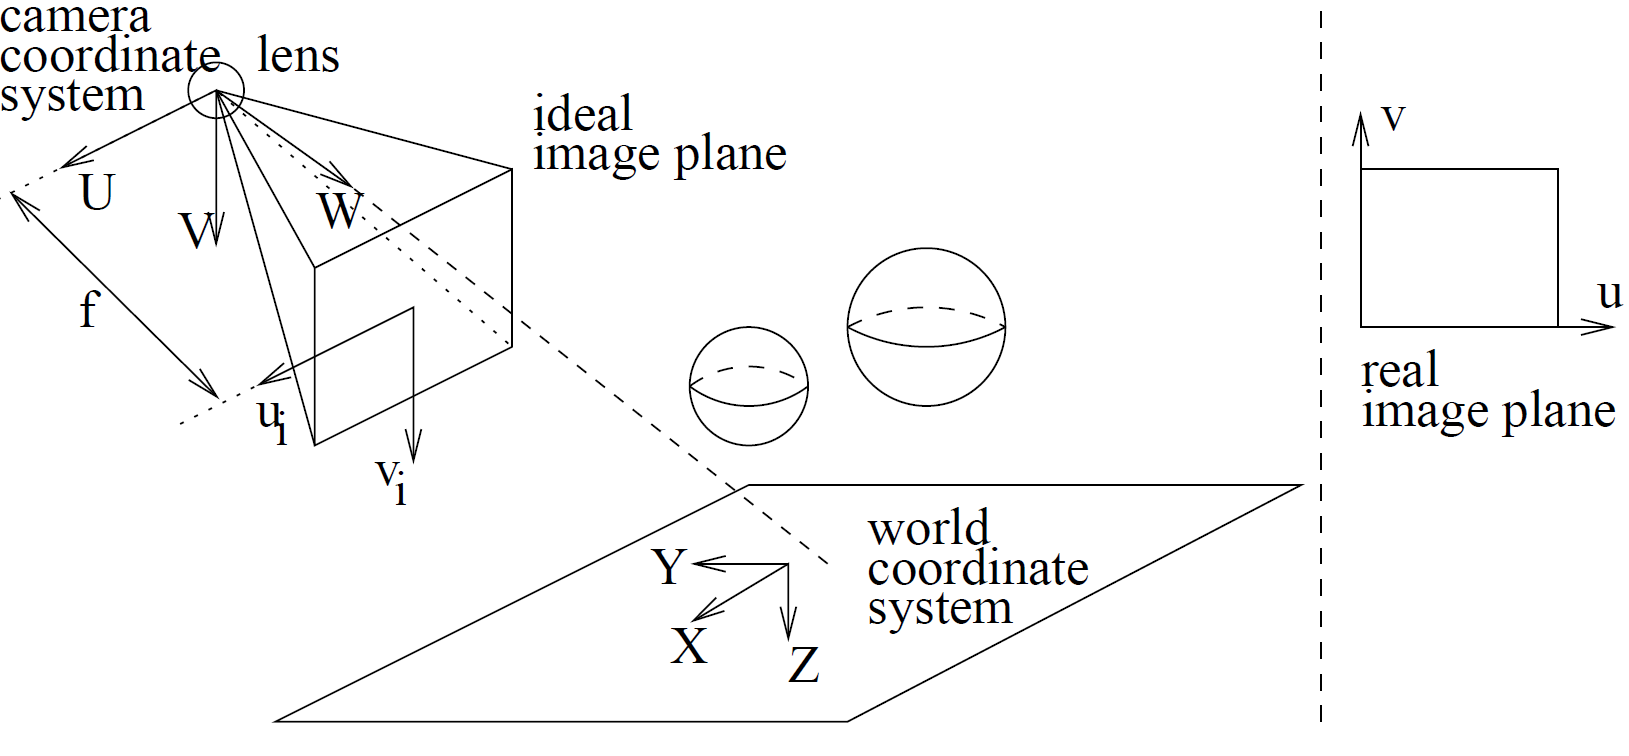
\includegraphics[width=\textwidth]{PinholeCameraModel}
\caption{The pinhole camera model}
\label{PinholeCameraModel}
\end{figure}%
%
\textbf{Extrinsic Calibration}\\
Without any camera parameters, the extrinsic calibration formula could be written, through homogeneous coordinates, as

\begin{equation}
%
\left[ \begin{array}{c} U \\ V \\ W \\ 1 \end{array} \right] %
= %
\begin{bmatrix} R & T \\ 0 & 1 \end{bmatrix} \times \left[ \begin{array}{c} X_w \\ Y_w \\ Z_w \\ 1 \end{array} \right]
%
\end{equation}%
%
or for simplicity,
\begin{equation}
%
\left[ \begin{array}{c} U \\ V \\ W \end{array} \right] %
= %
\begin{bmatrix} R & T \end{bmatrix} \cdot \left[ \begin{array}{c} X_w \\ Y_w \\ Z_w \end{array} \right]
\label{extrinsicTransform}
%
\end{equation}%
%
where \((U, V, W)^T\) are the camera coordinates, and the transformation matrix component \([R\)  \(T]\), which is part of the 4-by-4 perspective matrix, is modelling rotation and translation , written as

\begin{equation}
%
\left[ \begin{array}{cc} R & T \end{array} \right] %
= %
\begin{bmatrix}
 r_{11} & r_{12} & r_{13} & t_1 \\
 r_{21} & r_{22} & r_{23} & t_2 \\
 r_{31} & r_{32} & r_{33} & t_3
\end{bmatrix}
%
\end{equation}
\\\par
%
%
\textbf{Intrinsic Calibration}\\
Intrinsic Calibration could be separated into two sections. The first section is to rescale from camera coordinates to virtual ideal image coordinates. For a easier integration of two sections, the first section's formula is given through both of 2D coordinates to homogeneous coordinates.\par
%
\quad\quad2D coordinates:%
\begin{equation}
%
W \left[ \begin{array}{c} u_i \\ v_i  \end{array} \right] %
= f %
\left[ \begin{array}{c} U \\ V \end{array} \right]%
%
\end{equation}

\quad\quad Homogeneous coordinates:\par
\begin{equation}
%
W \left[ \begin{array}{c} u_i \\ v_i \\ 1 \end{array} \right] %
= %
\left[ \begin{array}{c} fU \\ fV \\ W \end{array} \right]%
=  \begin{bmatrix} f & 0 & 0 \\ 0 & f & 0 \\ 0 & 0 & 1 \end{bmatrix} \cdot %
\left[ \begin{array}{c} U \\ V \\ W \end{array} \right]%
\label{section_1}
\end{equation}%
\\\par
%
The second section is for translating and skewing between the virtual ideal image plane \(u_i\)/\(v_i\) and real image plane \(u_r\)/\(v_r\),  %

\begin{equation}
%
\left[ \begin{array}{c} u_r \\ v_r \\ 1 \end{array} \right] %
=  \begin{bmatrix} s_u & s_\theta & u_0 \\ 0 & s_v & v_0 \\ 0 & 0 & 1 \end{bmatrix} \cdot %
\left[ \begin{array}{c} u_i \\ v_i \\ 1 \end{array} \right]%
\label{section_2}
\end{equation}%
where \((u_0, v_0)\) denotes the optical center (or principal point), \([s_u, s_v]\) are skew coefficients in pixels along \(u\) and  \(v\) axes , and  \(s_\theta\) is an skewed angle generated by \(s_u\) and  \(s_v\). To combine equation \ref{section_1} and equation \ref{section_2}, we could get %

\begin{equation}
%
W \left[ \begin{array}{c} u_r \\ v_r \\ 1 \end{array} \right] %
=  \begin{bmatrix} s_u & s_\theta & u_0 \\ 0 & s_v & v_0 \\ 0 & 0 & 1 \end{bmatrix} \cdot%
 \begin{bmatrix} f & 0 & 0 \\ 0 & f & 0 \\ 0 & 0 & 1 \end{bmatrix} \cdot %
\left[ \begin{array}{c} U \\ V \\ W \end{array} \right]%
=  \begin{bmatrix} f_u & s & u_0 \\ 0 & f_v & v_0 \\ 0 & 0 & 1 \end{bmatrix} \cdot%
\left[ \begin{array}{c} U \\ V \\ W \end{array} \right]%
%
\label{intrinsicTransform}
\end{equation}%
%
where \([f_u,\, f_v]\) denote focal lengths in pixels along \(u\) and \(v\) after skewing, and \(s\) is a new skew coefficient after combination.\\\par%
%
\textbf{Generic Perspective Matrix of the Pinhole Camera Model}\par%
After both of the extrinsic and intrinsic transformation matrices have been derived, the generalization formula of the pinhole camera model could be derived, combining equation \ref{extrinsicTransform} and \ref{intrinsicTransform}, as

\begin{equation}
%
k \left[ \begin{array}{c} u_r \\ v_r \\ 1 \end{array} \right] %
=  \begin{bmatrix} f_u & s & u_0 \\ 0 & f_v & v_0 \\ 0 & 0 & 1 \end{bmatrix} \cdot%
\begin{bmatrix} R & T \end{bmatrix} \cdot \left[ \begin{array}{c} X_w \\ Y_w \\ Z_w \end{array} \right]%
=  C \cdot \left[ \begin{array}{c} X_w \\ Y_w \\ Z_w \end{array} \right]%
%
\end{equation}%
%
where \(W\) on the left side has been replaced by \(k\) to be a more general proportion coefficient, and a combined matrix can be expressed as
\begin{equation}
%
C %
=  \begin{bmatrix} f_u & s & u_0 \\ 0 & f_v & v_0 \\ 0 & 0 & 1 \end{bmatrix} \cdot%
\begin{bmatrix} R & T \end{bmatrix}%
= \begin{bmatrix} 
m_{11} & m_{12} & m_{13} & m_{14} \\
m_{21} & m_{22} & m_{23} & m_{24} \\
m_{31} & m_{32} & m_{33} & m_{34} \\
\end{bmatrix}%
%
\end{equation}%
%
The final 3-by-4 matrix C is considered as the generic perspective transformation matrix of a pinhole camera model, which gives a mapping between the 3D world coordinates and 2D real image coordinates.\par

\subsection{Lens distortion}
Lens distortion could be classified into two groups [10] : radial distortion, and tangential distortion.\par
%Z. Zhang, "Camera Calibration",   Chapter 2, pages 4-43, in G. Medioni and S.B. Kang, eds., Emergin Topics in Computer Vision, Prentice Hall Professional Technical Reference, 2004. .\par
%
Imperfect lens shape causes light rays bending more near the edges of a lens than they do at its optical center. The smaller the lens, the greater the distortion. Barrel distortions happen commonly on wide angle lenses, where the field of view of the lens is much wider than the size of the image sensor.\par%
Improper lens assembly will lead to tangential distortion, which occurs when the lens and the image plane are not parallel.\\\par
%
The lens distortion can be expressed as power series in radial distance \(r = \sqrt{x^2 + y^2}\):
\begin{equation}
%
\begin{aligned}
x_{distorted} =  x (1 + k_1 r^2 + k_2 r^4 + k_3 r^6) + [p_1 (r^2 + 2 x^2) + 2 p_2 xy] %
\\%
y_{distorted} =  y (1 + k_1 r^2 + k_2 r^4 + k_3 r^6) + [p_2 (r^2 + 2 y^2) + 2 p_1 xy]
\end{aligned}
\label{lensDistortion}
%
\end{equation}%

where higher order parameters are omitted for being negligible; \((x_{distorted}, \, y_{distorted})\) denote the distorted points, \((x, \, y)\) denote the undistorted pixel locations, \(k_i\)'s are coefficients of radial distortion, and \(p_j\)'s are coefficients of tangential distortion.\par
%
%%%%%%%%%%%%%%%%%%%%%%%%%%%%%%%%%%%%%%%%%%%%%%%%%%%%%%%
%%%%%%%%%%                                                     %%%%%%%%%%%%%%%%%%%%%%%%%%%
%%%%%%%%%%  1.3   Contributions of this thesis             %%%%%%%%%%%%%%%%%%%%%%%%
%%%%%%%%%%                                                     %%%%%%%%%%%%%%%%%%%%%%%%
%%%%%%%%%%%%%%%%%%%%%%%%%%%%%%%%%%%%%%%%%%%%%%%%%%%%%%%
\section{Contributions of this thesis}

%	****  Fourth order (abandon pinhole camera model) **********\\
%	****  Depth Rectification ************\\
%	****  Real-Time Reconstruction  ******\\
%	****  accurate calibration system *******\\\\\par
	
For RGB-D cameras, RGB steam and Depth steam are two steams that independent but correlated with each other. With respect to every \(X_{w}\) /\(Y_{w}\)  correlated single pixel-pair, Depth steam offers the additional voxel world coordinates \(Z_{w}\) , while RGB steam offers the additive color property.
\\
\\As described in section \ref{sens_TraditionalCalibration}, the traditional way to reconstruct 3D point cloud not only has the time-cost problem, but also makes \(Z_{w}\) accuracy unguaranteed. First of all, the lens distortions correction is separated from pinhole camera model calibration. Even though same pixel-pair's of world coordinates and image plan coordinates could be reused to solve radial dominated lens distortions, the calculation of the separated step brings a second-time translation cost for every single pixel of every frame. This is not a good way to do real-time reconstruction. What's worse, the depth resolution deteriorates notably with depth in practical [11],
%Consumer RGB-D Cameras and their Applications, by Krystof Litomisky
 and noises among depth data vary randomly, camera by camera and pixel by pixel; which means a rough point-cloud plane full of bumps and hollows will be reconstructed even though the camera is observing a wall. Like figure 1.8 shows%
\\\\Figure 1.8: side face of a sags and crests RGB plane 
\\\\
\\In General, a rectification of 3D coordinates \(X_{w}\) /\(Y_{w}\) /\(Z_{w}\)  for every single pixel is needed to get a better view of a target's 3D profile. In this thesis, instead of using model based traditional method, an accurate data based  \(X_{w}\) /\(Y_{w}\) /\(Z_{w}\) rectified real-time reconstruction method is proposed. In Chapter 2, \(X_{w}\) and \(Y_{w}\) are rectified separately through a fourth order surface fitting translation from image plane row and column to directly solve the lens distortion problem in equation \ref{lensDistortion}, considering that the parameters in that equation with power level larger than 4 are negligible. Then, \(Z_{w}\) values are totally supported from external BLE optical-flow sensor, which accurately tracks camera movements along Z-axis. Finally, a XYZWRGB-D model based lookup table will be generated for real-time reconstruction. Whole calibration system will be introduced in detail in Chapter 3. Results will be shown in Chapter 4.





\section{Summation}













































